\graphicspath{ {../images/}}

\chapter{Preliminaries}\label{ch:preliminaries}
In this chapter, we will introduce all the necessary mathematical and quantum concepts that will be used throughout this thesis. It is important to understand these concepts before we proceed further. We will begin by covering fundamental mathematical concepts, followed by quantum computing concepts. Finally, we will cover Hamiltonian and ground state energy, these concepts are also somewhat intertwined with chemistry.

\section{Mathematics of quantum computing}
In the case of standard computers, boolean algebra is used. Quantum computing leverages the power of linear algebra. In this section, we will introduce concepts from linear algebra and some concepts that are more specific to physics. We heavily rely on definitions from the book Mathematical Methods for Physicists by Arfken et al.~\cite{mmp}.

\subsection*{Eigenvalues and eigenvectors}
Eigenvalues and eigenvectors are some of the most important concepts in linear algebra. The problem of eigenvalues and eigenvectors can be defined by the following equation:

\begin{equation}
  A\vec{v} = \lambda \vec{v}\text{,}
  \label{eq:eigen}
\end{equation}

\noindent where $A$ is a square matrix, vector $\vec{v}$ and constant $\lambda$ are unknown. If $\vec{v} \neq 0$, $\vec{v}$ is an eigenvector of matrix $A$. Each eigenvector has a corresponding eigenvalue $\lambda$. Equation~\ref{eq:eigen} shows that the resulting vectors after multiplication with matrix $A$ and constant $\lambda$ are equal. That necessarily means that an eigenvector of a matrix is a vector that does not change its direction when multiplied by that matrix, only its length changes. An eigenvalue is a scalar representing how much the eigenvector is stretched or shrunk. This concept can be easily visually interpreted, see Figure~\ref{fig:eigen}.

\begin{figure}[H]
  \centering
  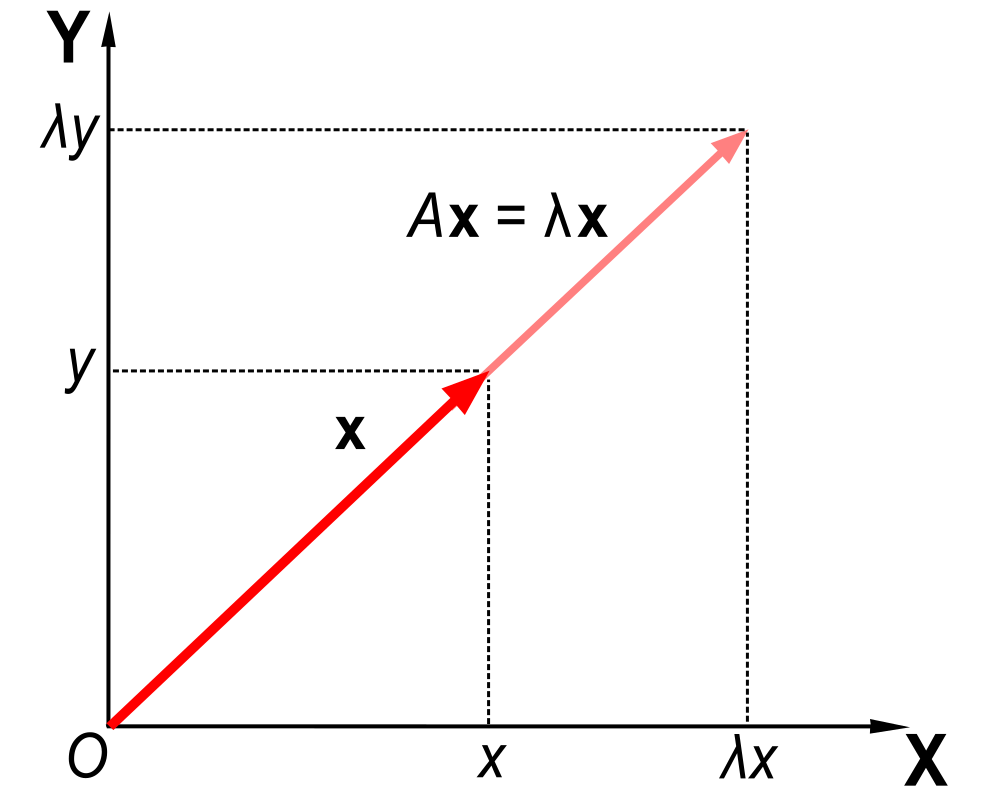
\includegraphics[width=0.5\textwidth]{eigenvector.png}
  \caption{Geometric interpretation of eigenvectors and eigenvalues \cite{img:eigen}}
  \label{fig:eigen}
\end{figure} 

\subsection*{Complex conjugate}
A complex number consists of real and imaginary parts, where the imaginary unit satisfies the equation $i^2 = -1$. If we have a complex number $z = a + bi$, its complex conjugate is $z^{*} = a - bi$. The imaginary part has just flipped the sign. 
\begin{equation}\label{eq:complex-conjugate}
zz^{*} = (a + bi)(a - bi) = a^2 - (bi)^2 = a^2 + b^2
\end{equation}
Equation \ref{eq:complex-conjugate} reveals that $zz^{*}$ is a non-negative real number and it enables us to define absolute value as $\sqrt{zz^{*}}$, which is denoted by $\lvert z \rvert$. A complex conjugate can be also denoted as $\bar{z}$.

\subsection*{Adjoint of a matrix}
For matrices with complex elements, the complex conjugate of a matrix is obtained by conjugating all elements of the original matrix. The notation for the complex conjugate of $A$ is $A^*$. The adjoint of a matrix $A$, denoted $A^\dag$ ($A$ dagger), is obtained by both complex conjugating and transposing it. The adjoint of real matrices is just equal to their transpose.

\subsection*{Unitary matrices}
Unitary matrices are matrices that satisfy the property $U^\dag = U^{-1}$, meaning their adjoint equals their inverse. The relationship can be also expressed as follows:
\begin{equation}
U U^{\dag} = U^{\dag} U\text{.}
\end{equation}
Also, provided that $U$ and $V$ are both unitary, then $UV$ and $VU$ will be unitary as well.

\subsection*{Hermitian matrices}
A definition of Hermitian matrices builds upon the previous definitions. Hermitian matrices are square matrices that are equal to their adjoint, therefore $H = H^\dag$. Synonymously, they are also called self-adjoint matrices. All real symmetric matrices are Hermitian. It is important to note that if two matrices $A$ and $B$ are Hermitian, there is no guarantee that either $AB$ or $BA$ will also be Hermitian. It is guaranteed that Hermitian matrices have real eigenvalues.

\subsection*{Pauli matrices}\label{sec:pauli-matrices}
By Pauli matrices, we mean the set of three $2 \times 2$ complex matrices. They are defined as follows:
\begin{equation*}
  \sigma_X = \begin{pmatrix}
    0 & 1 \\
    1 & 0
 \end{pmatrix}, \sigma_Y = \begin{pmatrix}
    0 & -i \\
    i & 0
\end{pmatrix}, \sigma_Z = \begin{pmatrix}
    1 & 0 \\
    0 & 1
\end{pmatrix}\text{.}
\end{equation*}
These matrices are both Hermitian and unitary. Some literature also includes the identity matrix in the set of Pauli matrices. 

\subsection*{Tensor product}
The tensor product is an operation that is heavily used in quantum computing. It is a general operation that applies to several mathematical objects, but in this case, we will restrict ourselves to matrices. The version that works for matrices can be referred to as the Kronecker product. Sometimes are these operations used interchangeably since they use the same notation $\otimes$. Essentially, it is a binary operation that combines two matrices into one larger matrix. We multiply each element of the first matrix by the entire second matrix. Mathematically, it is defined as follows:
\begin{equation*}
  A \otimes B = \begin{pmatrix}
    a_{11}B & a_{12}B & \hdots & a_{1n}B \\
    a_{21}B & a_{22}B & \hdots & a_{2n}B \\
    \vdots & \vdots & \ddots & \vdots \\
    a_{m1}B & a_{m2}B & \hdots & a_{mn}B
  \end{pmatrix}\text{.}
\end{equation*}

\subsection*{Bra-ket notation}
Bra-ket notation, also known as Dirac notation plays an important role in quantum mechanics. It is a notation for vectors used to describe a quantum state. A ket is a standard column vector whereas a bra is an adjoint of a ket. 

\begin{table}[H]
  \centering
  \begin{tabular}{ c @{\hspace{3cm}} c }
        $\bra{\alpha} = \begin{pmatrix}
            a_1^* & a_2^* & \hdots & a_n^*
        \end{pmatrix}$ & $\ket{\beta} = \begin{pmatrix}
            b_1 \\
            b_2 \\
            \vdots \\
            b_n
        \end{pmatrix}
        $ \\ 
         & \\
     Bra & Ket
  \end{tabular}
\end{table}

The main advantage of this notation is that enables us to easily write vector operations such as inner product:
\begin{equation*}
  \braket{\alpha}{\beta} = \begin{pmatrix}
    a_1^* & a_2^* & \hdots & a_n^*
\end{pmatrix}\begin{pmatrix}
    b_1 \\
    b_2 \\
    \vdots \\
    b_n
\end{pmatrix} = \sum_{i=1}^{n} a_i^{*} b_i\text{,}
\end{equation*}
outer product:
\begin{equation*}
  \ket{\beta}\bra{\alpha} = \begin{pmatrix}
    b_1 \\
    b_2 \\
    \vdots \\
    b_n
\end{pmatrix}
\begin{pmatrix}
    a_1^* & a_2^* & \hdots & a_n^*
\end{pmatrix} = \begin{pmatrix}
    b_{1}a_1^* & b_{1}a_2^* & \hdots & b_{1}a_n^* \\
    b_{2}a_1^* & b_{2}a_2^* & \hdots & b_{2}a_n^* \\
    \vdots & \vdots & \ddots & \vdots \\
    b_{n}a_1^* & b_{n}a_2^* & \hdots & b_{n}a_n^*
\end{pmatrix}\text{,}
\end{equation*} and tensor product:
\begin{equation*}
  \ket{\alpha} \otimes \ket{\beta} = \ket{\alpha}\ket{\beta} = \ket{\alpha \beta}\text{.}
\end{equation*}

\subsection*{Hilbert space}
Mostly, we used to work with finite-dimensional vector spaces. Recall that the dimension of vector space is the number of vectors required to form a basis. In quantum computing, we work with infinite-dimensional vector spaces over field $\mathbb{C}$. Virtually, Hilbert space $\mathcal{H}$ is a standard vector space over $\mathbb{C}$, but in addition to that it satisfies the property of completeness:
\begin{equation*}
  \sum_{i=0}^{\infty}\vert a_i \vert \in \mathcal{H}\text{.}
\end{equation*}
Simply put, each Cauchy sequence of vectors converges to a vector that lies in Hilbert space $\mathcal{H}$.

\ques{Neviem, ta definicia sa mi moc nepozdava. Je to pochopitelne?}

\section{Introduction to quantum computing}
The standard computers as we know them, for their functioning use laws of standard mechanics. Quantum computers, on the other hand, use the laws of quantum mechanics. Quantum mechanics describes the behavior of particles at the microscopic level, whereas standard mechanics deals with macroscopic objects. The objective of this section is to highlight the most important concept and provide at least a brief idea of quantum computing. The main source of information for this section is the book Quantum Computation and Quantum Information by Michael A. Nielsen and Isaac L. Chuang~\cite{qc}.

\subsection*{Qubit}
A qubit is an abbreviation of a quantum bit. It is a bit counterpart in quantum computing, thus a basic unit of information in quantum computers. Classical bits can hold only two values, either 0 or 1. However, qubits are more complex.

Mathematically, a qubit is represented by a vector in a two-dimensional complex vector space. Basis vectors of this vector space:
\begin{equation*}
\ket{0} = \begin{pmatrix} 1 \\ 0 \end{pmatrix}\text{ and }\ket{1} = \begin{pmatrix} 0 \\ 1 \end{pmatrix}
\end{equation*}
are also known as computational basis states and they are analogous to classical bits 0 and 1. In addition, qubits can be in a so-called superposition of states. This means that a state of a qubit can be a linear combination of states $\ket{0}$ and $\ket{1}$:
\begin{equation*}
\ket{\psi} = \alpha \ket{0} + \beta \ket{1}\text{, where } \alpha,\beta \in \mathbb{C}\text{, and } \lvert \alpha \rvert^2 + \lvert \beta \rvert^2 = 1\text{,}
\end{equation*}
therefore there are infinitely many states that qubit can be in. In case we consider two qubits, the basis vectors of this four-dimensional vector space are $\ket{00}$, $\ket{01}$, $\ket{10}$, and $\ket{11}$. Then the superposition looks as follows:
\begin{equation*}
 \ket{\psi} = \alpha \ket{00} + \beta \ket{01} + \gamma \ket{10} + \delta \ket{11}\text{,}
\end{equation*}
where the sum of the squared coefficients is equal to 1 as well. 

All these vectors and complex numbers may be difficult to understand and imagine. For simplification, we can leverage the Bloch sphere to visualize the state of a qubit. It is a unit sphere named after physicist Felix Bloch. For the sake of simplicity, we will not go into the details, but if we use the properties of a quantum state, there is a possibility to rewrite it cleverly, such that a quantum state can be visualized as a vector in a Bloch sphere.

\begin{figure}[H]
    \begin{center}
       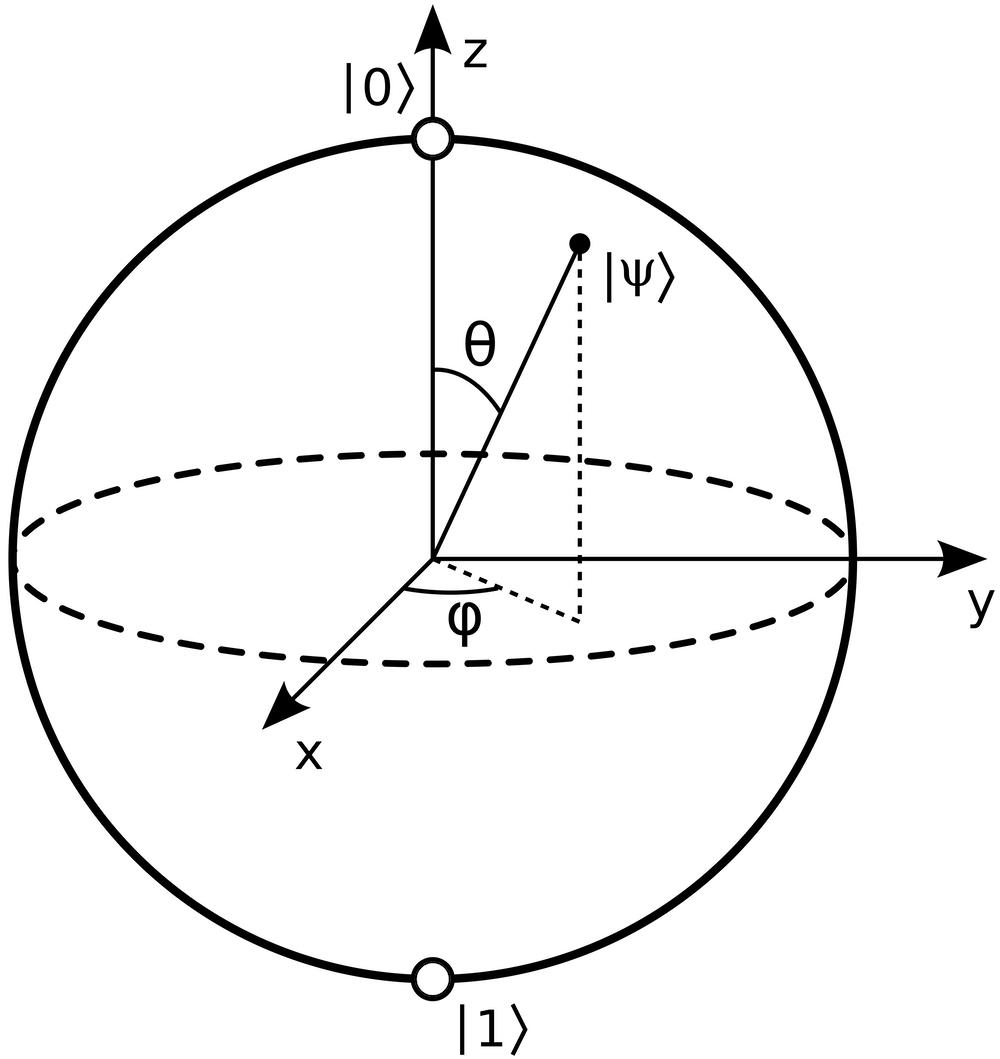
\includegraphics[width=0.5\textwidth]{bloch-sphere.png}
       \caption{Bloch sphere \cite{img:bloch_sphere}}
    \end{center}
\end{figure} 

This was just a mathematical representation, however, in the real world physical qubits can be realized in different ways. There is a plethora of options but the most prominent ones used by leading companies are superconducting qubits and trapped ions (an atom that is not neutral). Also, we cannot omit photon-based qubits that can succeed as well.  

\subsection*{Measurements}
Measurement is an operation that enables us to find out the state of a qubit, however, this operation does not work as most of us would expect. When a qubit is measured, it yields either outcome $\ket{0}$, with a probability of $\lvert \alpha \rvert^2$, or outcome $\ket{1}$, with a probability of $\lvert \beta \rvert^2$. We are working with probabilities, so the normalization condition $\lvert \alpha \rvert^2 + \lvert \beta \rvert^2 = 1$, should make more sense now. Measurement is a destructive operation, upon first measurement, the state of a qubit is collapsed to either $\ket{0}$ or $\ket{1}$, and any subsequent measurements will yield the same result. We cannot recover the original state of a qubit after measurement. Table~\ref{tab:measurements-states} shows canonical measurements on the x, y and z axes, however, there are infinitely many ways to measure a qubit, depending on how we rotate it.

\begin{table}[H]
  \centering
  \begin{tabular}{|c|c|} 
      \hline
      \multicolumn{1}{|c|}{\textbf{Measurement axes}} & \textbf{States}\\
      \hline
      x-axis & $\ket{+} \text{ and }\ket{-}$\\ 
      \hline
      y-axis & $\ket{-i} \text{ and }\ket{+i}$\\ 
      \hline
      z-axis & $\ket{0} \text{ and }\ket{1}$\\ 
      \hline
  \end{tabular}
  \caption{Mesaurements and their respective states}
  \label{tab:measurements-states}
\end{table}
Most (if not all) contemporary quantum computers perform measurements only on a computational basis (z-axis)~\cite{blog}. Table~\ref{tab:measurements-conversion} demonstrates how measurements on the x and y axes can be converted to the z-axis measurement.
\begin{table}[H]
  \centering
  \begin{tabular}{|c|c|} 
      \hline
      \multicolumn{1}{|c|}{\textbf{Measurement axes}} & \textbf{Conversion}\\
      \hline
      x-axis & we apply gate $RY(-\pi/2)$ \\ 
      \hline
      y-axis & we apply gate $RX(\pi/2)$ \\ 
      \hline
  \end{tabular}
  \caption{Measurements and their conversion to computational basis}
  \label{tab:measurements-conversion}
\end{table}

\subsection*{Quantum gates}
Thus far, our focus has been on examining the properties of qubits, leaving the question of qubit manipulation unanswered. This section delves into the fundamental quantum gates, accompanied by visual representations to enhance comprehension.

Quantum gates are the quantum equivalent of classical logic gates. In contrast to logic gates in classical computing, quantum gates are represented by matrices. The only property that a matrix must adhere to is unitarity. There are infinitely many unitary matrices, therefore we have infinitely many quantum gates.

Another specialty of quantum gates or quantum computation is their reversibility. This means that from the output of the gate, we can always determine the input. This is not the case for logic gates. For instance, the \textit{AND} gate is not reversible. From the output, we cannot determine the input.

\subsubsection*{X, Y, Z gates}
Gates X, Y, and Z are the most fundamental single-qubit gates. All three gates perform rotation by 180 degrees of the Bloch sphere \ques{I would say rotation of a state}, the X gate around the x-axis, the Y gate around the y-axis, and the Z gate around the z-axis. They are also known as bit-flip, phase-flip, and bit-phase-flip gates, respectively. Parametrized equivalents of these gates are called RX, RY, and RZ. These gates are used to rotate the state of a qubit by a given angle.

\begin{table}[H]
  \centering
  \begin{tabular}{|c|c|c|} 
      \hline
      \textbf{X-gate} & \textbf{Y-gate} & \textbf{Z-gate}\\
      \hline
      &&\\[0.5pt]
      $\begin{pmatrix}
        0 & 1 \\
        1 & 0
      \end{pmatrix}$ & 
      $\begin{pmatrix}
        0 & -i \\
        i & 0
      \end{pmatrix}$ &
      $\begin{pmatrix}
        1 & 0 \\
        0 & -1
      \end{pmatrix}$\\
      &&\\[0.5pt]
      \hline
      &&\\[0.5pt]
      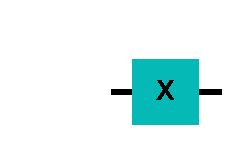
\includegraphics[]{gate-x.pdf} & 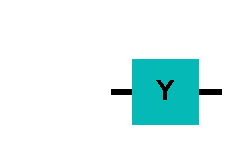
\includegraphics[]{gate-y.pdf}  & 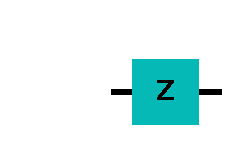
\includegraphics[]{gate-z.pdf}\\
      &&\\[0.5pt]
      \hline
      &&\\[0.5pt]
      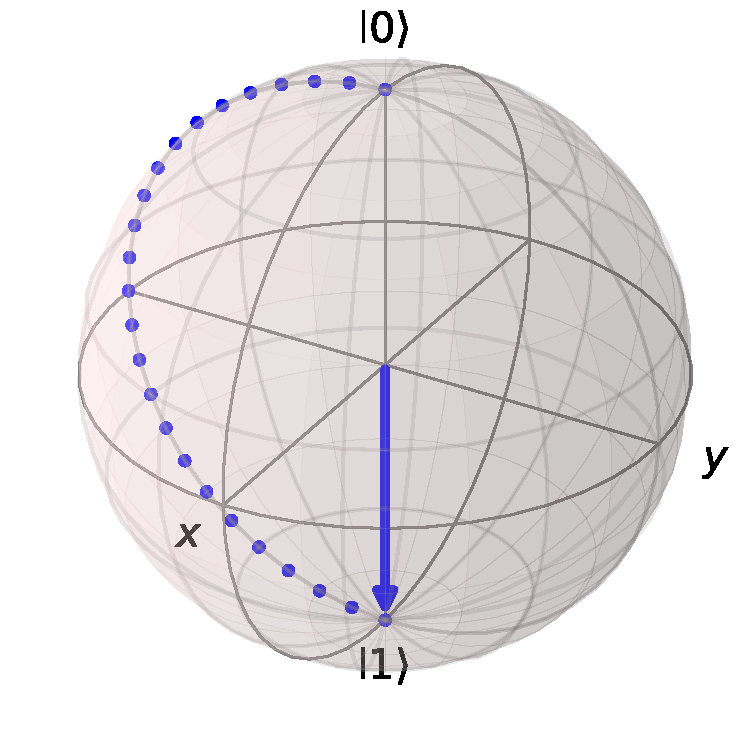
\includegraphics[width=.32\textwidth]{qubit-x-gate.pdf} & 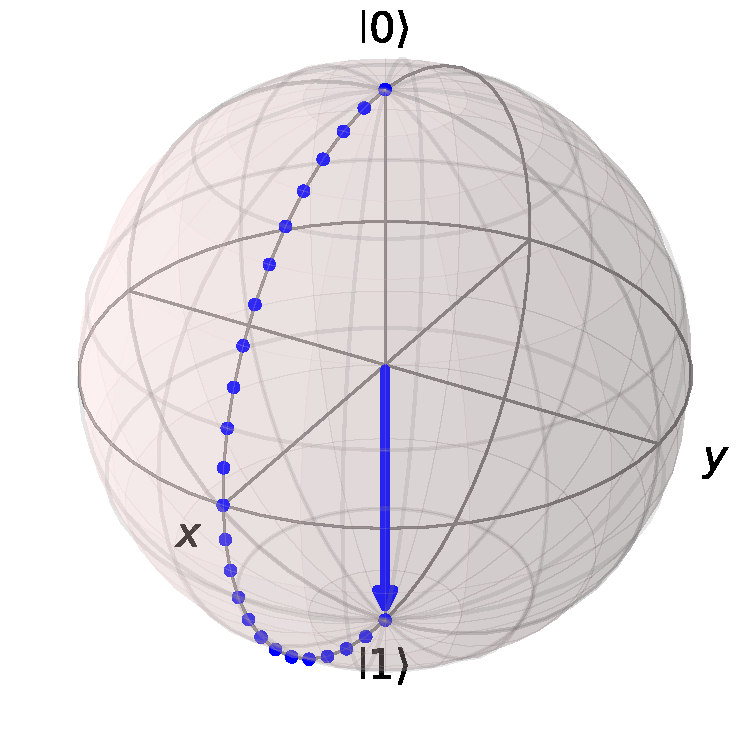
\includegraphics[width=.32\textwidth]{qubit-y-gate.pdf} & 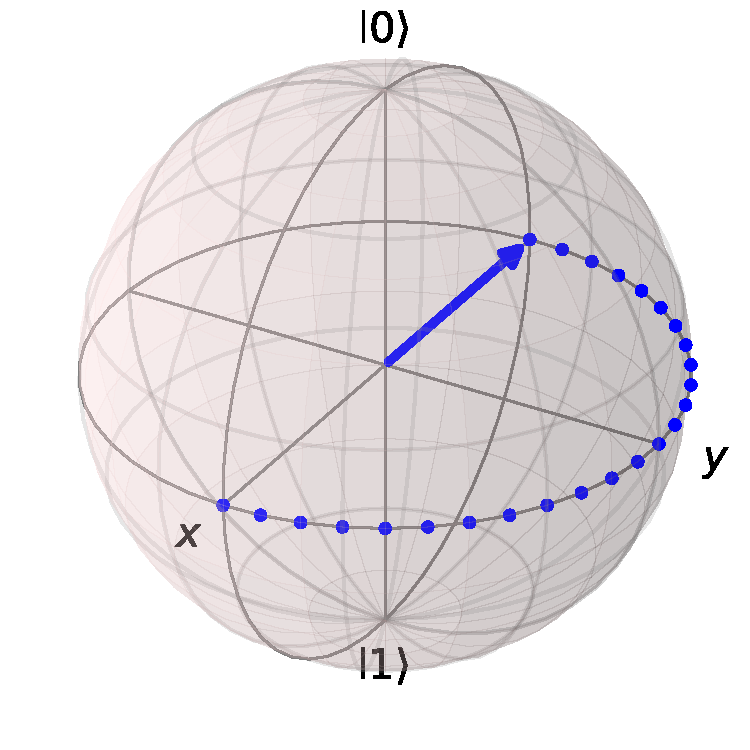
\includegraphics[width=.32\textwidth]{qubit-z-gate.pdf}\\
      \hline
  \end{tabular}
  \caption{X, Y, and Z gates and their representations}
  \label{tab:xyz-gates}
\end{table}
Note that the initial state of the Z-gate differs from the initial state of the X and Y gates. If we had started from the state $\ket{0}$, we would have not seen any change.

\subsubsection*{Hadamard gate}
The Hadamard operation can be thought of as a two-step process. It is a rotation of the sphere around the y-axis by 90 degrees and then subsequent rotation around the x-axis by 180 degrees. If we apply Hadamard gate on a qubit in the state $\ket{0}$, we get a qubit in an equal superposition of states $\ket{0}$ and $\ket{1}$.
\begin{figure}[H]
    \centering
    \begin{minipage}{0.4\linewidth}
      \centering
      $\begin{pmatrix} 
        \frac{1}{\sqrt{2}} &  \frac{1}{\sqrt{2}}  \\
        \frac{1}{\sqrt{2}}  &  -\frac{1}{\sqrt{2}} 
        \end{pmatrix}$
    \end{minipage}
    \begin{minipage}{0.25\linewidth}
      \centering
      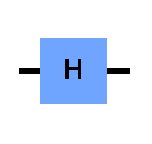
\includegraphics[scale=0.8]{gate-hadamard.pdf}
    \end{minipage}
    \caption{Hadamard gate representation}
\end{figure}

\subsubsection*{Controlled-NOT gate} 
Controlled-NOT (CNOT) gate operates on two input qubits, known as the control qubit and the target qubit. The action of the gate may be described as follows. If the control qubit is set to state $\ket{0}$, then the target qubit remains untouched. Conversely, if the control qubit is set to state $\ket{1}$, then the target qubit is flipped.

\begin{figure}[H]
  \centering
  \begin{minipage}[c]{0.4\linewidth}
    \centering
    $$\begin{pmatrix}
      1 & 0 & 0 & 0 \\
      0 & 1 & 0 & 0 \\
      0 & 0 & 0 & 1 \\
      0 & 0 & 1 & 0
  \end{pmatrix}$$
  \end{minipage}
  \begin{minipage}[c]{0.25\linewidth}
    \centering
    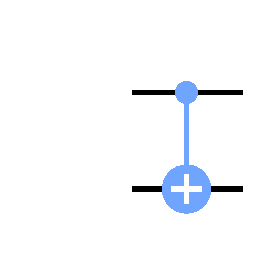
\includegraphics[scale=0.8]{gate-cnot.pdf}
  \end{minipage}
  \caption{CNOT gate representation}
\end{figure}

\subsection*{Quantum entanglement}
Apart from superposition, quantum entanglement is another quantum phenomenon that gives us an advantage over classical computers. When qubits are entangled we mean that they are somehow bound together and they are dependent. Altering the state of one qubit will immediately alter the state of the other qubit predictably. In the below example, we will demonstrate the most simple entangled state, also known as the Bell state.

\begin{figure}[H]
\begin{minipage}{.5\textwidth}
    \centering
    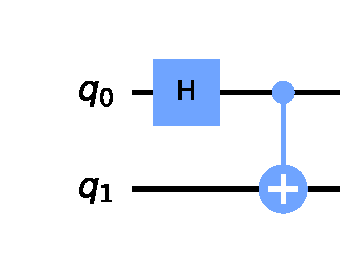
\includegraphics[]{entanglement-circuit.pdf}
    \caption{Bell state circuit}
\end{minipage}
\begin{minipage}{.5\textwidth}
  \begin{align} 
             &\ket{00} = \ket{0} \otimes \ket{0} \label{eq1} \\
             &\frac{1}{\sqrt{2}}(\ket{0} + \ket{1}) \otimes \ket{0} \label{eq2}\\
             &\frac{1}{\sqrt{2}}(\ket{0} \otimes \ket{0} + \ket{1} \otimes \ket{0}) \label{eq3} \\
             &\frac{1}{\sqrt{2}}(\ket{0} \otimes \ket{0} + \ket{1} \otimes \ket{1}) \label{eq4}\\
             &\frac{1}{\sqrt{2}}(\ket{00} + \ket{11}) \label{eq5}
  \end{align}
\end{minipage}
\end{figure}

\noindent In the following lines, we explain individual steps of the computation.\\
\noindent (\ref{eq1}) Initial state of the circuit.\\
(\ref{eq2}) Hadamard gate applied, the first qubit is equally likely to be in state $\ket{0}$ or $\ket{1}$.\\
(\ref{eq3}) Expanded bracket.\\
(\ref{eq4}) CNOT gate applied, the first qubit is $\ket{1}$, state of the second qubit will be flipped.\\
(\ref{eq5}) Final state of the circuit.\\

\noindent From the above example, we can see that the qubits are correlated. This particular state is a superposition only of two states $\ket{00}$ and $\ket{11}$, without entanglement we would have to consider a superposition of four states $\ket{00}$, $\ket{01}$, $\ket{10}$, and $\ket{11}$. If the first qubit is measured to be in state $\ket{0}$, then the second one will also be in state $\ket{0}$. The same applies to state $\ket{1}$.

\subsection*{Noisy Intermediate-Scale Quantum (NISQ) computers}
In today's world, quantum computers still suffer from several problems, namely the following ones.

\subsubsection{Scalability}
The more qubits we have, the bigger instances of problems we can solve. However, with an increasing number of qubits and a number of gates we introduce errors into quantum computation. The gates themselves, especially the entangling ones, possess a certain probability that the outcome of the gate will result in an error. Also, qubit connectivity goes hand in hand with the scalability. It is not very rational to have many qubits if they are not connected and we cannot use multiqubit gates on them.

\subsubsection{Quantum decoherence}
Qubits are very sensitive and their state can be easily influenced by the noise from the environment. By noise we mean magnetic fields, radio waves, vibrations, light, and more. To minimize this effect, quantum processing units (QPUs) are accompanied by other components that are used to shield the qubits from the environment and keep them at temperatures close to absolute zero ($0$K = $-273.15^{\circ}$C). Thanks to that, quantum computers are large in size and they often resemble chandeliers even though QPUs are in size comparable to processors in standard computers.

\subsubsection{Lack of error correction}
Theoretically, we always consider so-called logical qubits that do not have any problems and work seamlessly. In reality, we use physical qubits that suffer from noise and decoherence and it hinders us from executing quantum algorithms reliably. To mitigate this problem, we can use quantum error correction. The idea is that we can use multiple physical qubits, from tens even to thousands, to create a single reliable logical qubit. By doing so we run into a problem with scalability. 

\paragraph{}
Quantum computers that match these characteristics are called noisy intermediate-scale quantum (NISQ) computers. These characteristics and the term NISQ were introduced by John Preskill~\cite{nisq} and its meaning is the following. The term ``noisy'' refers to all the noise that quantum computers currently suffer from. The noise will significantly constrain the capabilities of quantum computers in the foreseeable future. ``Intermediate-scale'' denotes the quantum computers expected to emerge in the coming years, featuring a qubit count ranging from 50 to a few hundred. 

\section{Ground state energy}
Before getting into the ground state energy, let's revisit an atom first. Atoms are the smallest building blocks of matter~\cite{chemistry}. They are composed of 3 subatomic particles, protons, neutrons, and electrons. Protons and neutrons are located within the nucleus of the atom. As their names suggest, protons have a positive electrical charge, while neutrons are electrically neutral. Electrons have a negative electrical charge. Atoms themselves are neutral, so the number of protons must be equal to the number of electrons. Electrons are attracted to the protons in the nucleus by the electrostatic force that exists between particles of opposite electrical charge.

Electrons are organized into orbitals, each with its own characteristic shape and energy level~\cite{chemistry}. An electron has the ability to transition between orbitals by either absorbing or emitting photons with energy precisely matching the difference in energy between the two orbits. In order for the electron to transition to a higher-energy state, it must absorb energy. Conversely, energy is emitted when the electron transitions to a lower-energy state. The lowest-energy state is also known as the ground state and higher-energy states are called excited states. We will measure this energy in the Hartree (Ha) units. Hartree is a unit of energy in the atomic units system~\cite{hartree}.

\ques{Oba odseky su parafrazovane z tej chemickej knihy. Nie som uplne spokojny ako to je vyznacene, asi nie je uplne jasne, ze ta parafraza pokracuje aj po vete v ktorej sa uviedla referencia. Ako by som to mohol zlepsit?}

\begin{figure}[H]
    \centering
    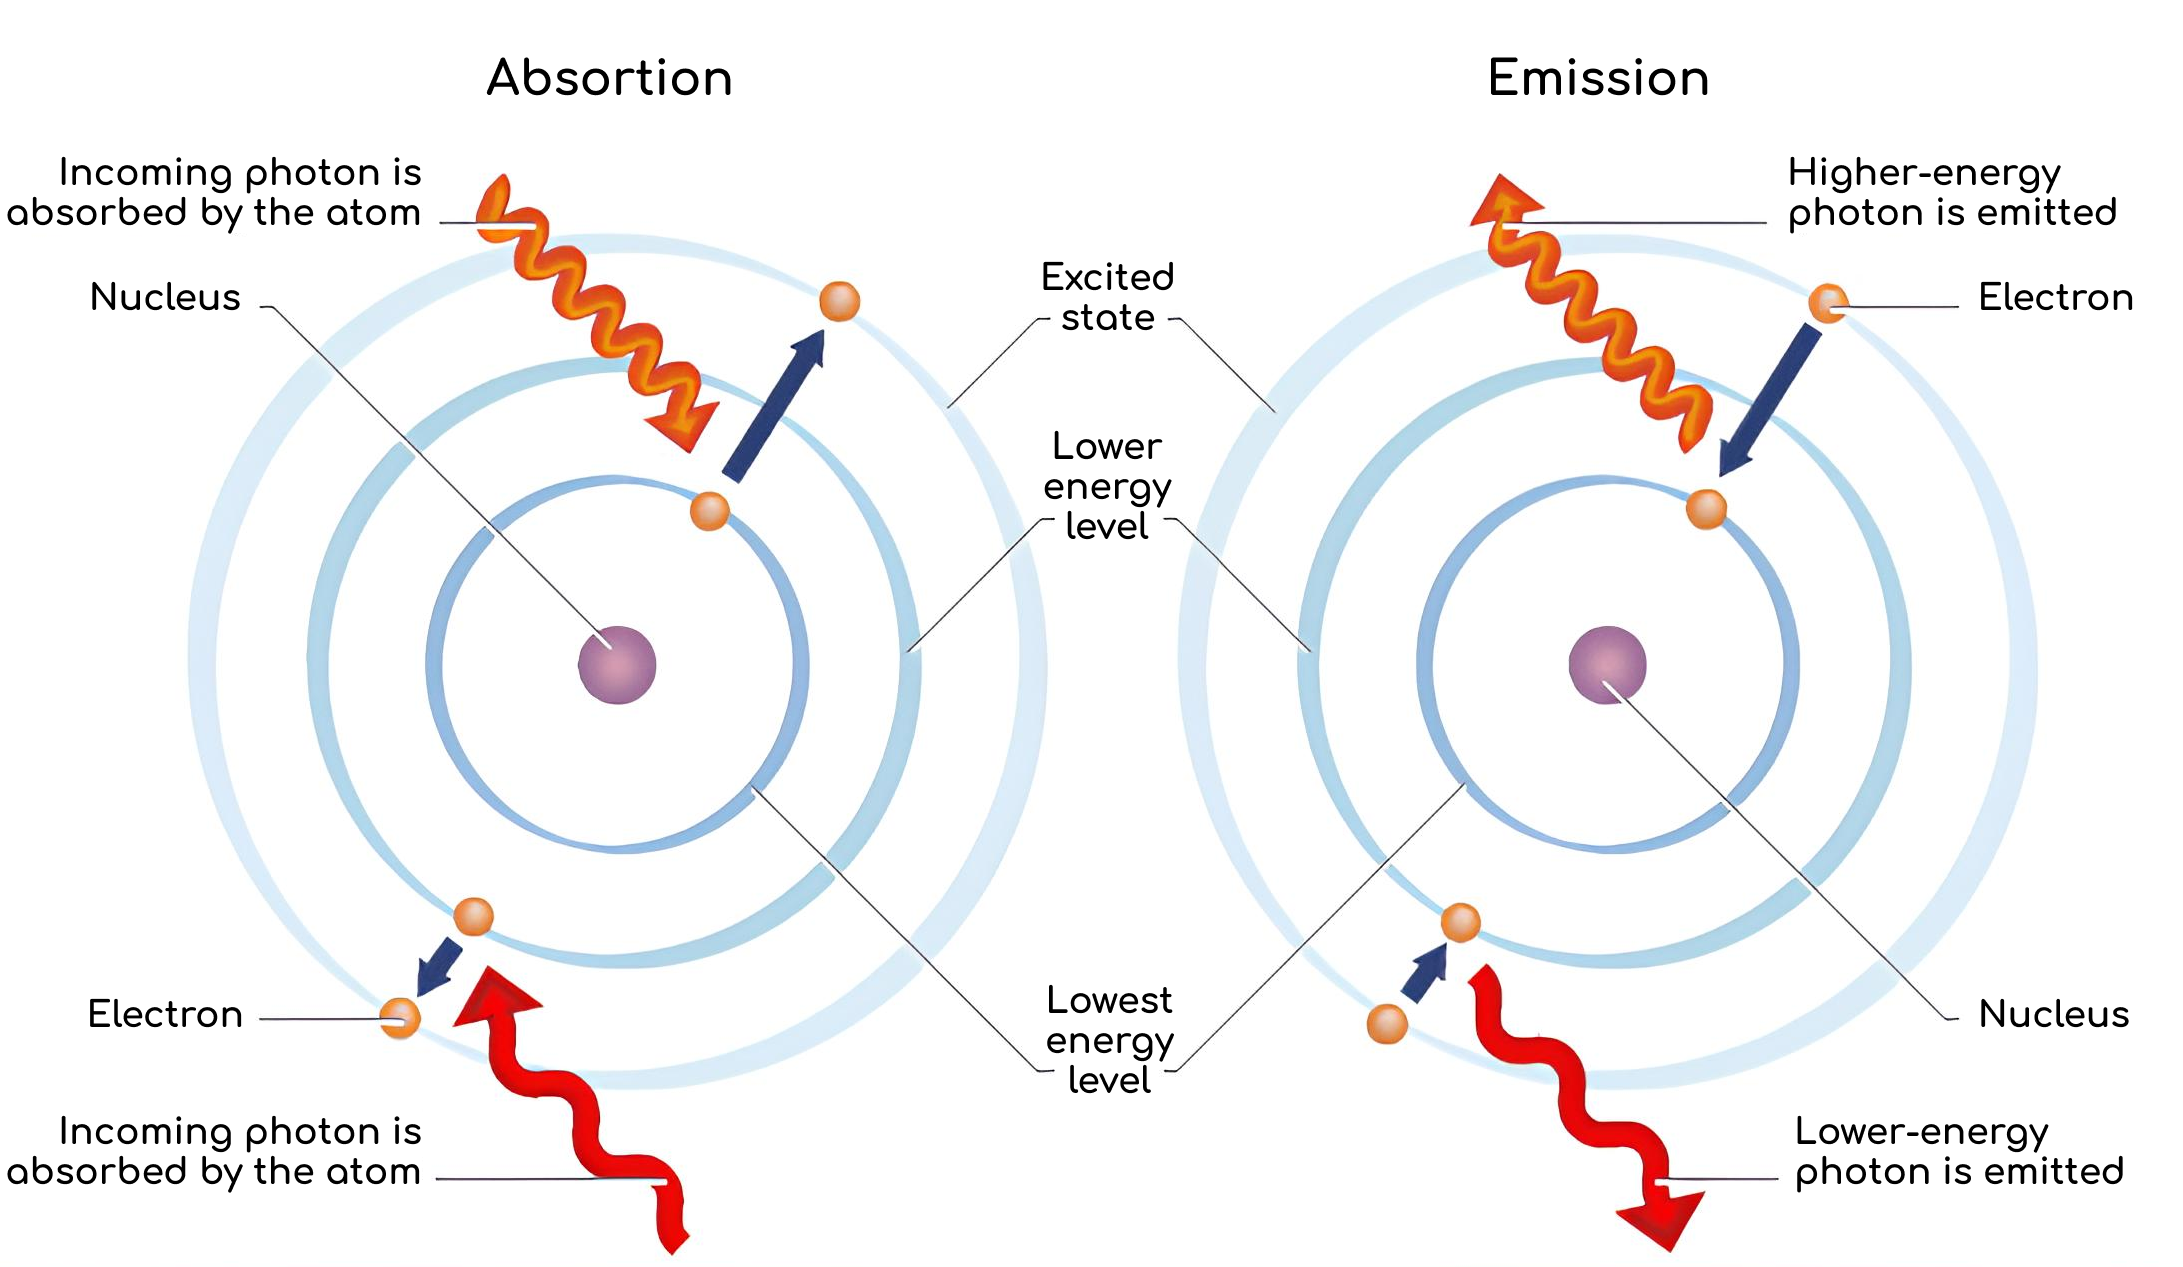
\includegraphics[width=\textwidth]{ground-state.png}
    \caption{Absorption and emission of a photon by an electron~\cite{img:ground-state}}
\end{figure}

\section{Hamiltonian}
The Hamiltonian defines the total energy of a physical system. Many different forms of Hamiltonians exist in physics and chemistry, but for us, it is just a matrix. Once a Hamiltonian is constructed, it must be translated into operators that can be directly measured on a quantum computer. The representation for quantum computers looks as follows~\cite{ibm_hamiltonian}:
\begin{equation*}
\hat{H} = \sum_{i=1}^{m}c_i\sigma_i \text{, } \sigma_i \in \{I, X, Y, Z\}^{\otimes n}\text{, } c_i \in \mathbb{R} \text{, }
\end{equation*}
where $I$ is an identity matrix and $X$, $Y$, $Z$ are Pauli matrices which we discussed in the section~\ref{sec:pauli-matrices}.

The Pauli matrices represent measurements. For instance, the expression $c_{1}Z_{0}X_{1}Y_{2}$ means that we measure qubit zero on the z-axis, qubit one on the x-axis, qubit two on the y-axis, and then we will multiply the results together with the coefficient $c_{1}$. Sometimes this Hamiltonian representation is referred to as a sum of Pauli strings. A ground state energy is a real number therefore this Hamiltonian representation has real eigenvalues, this fact concludes that Hamiltonian is a Hermitian matrix.